\section{EXPERIMENTS}\label{results}

\subsection{Comparison with the Virtual Hitting Plane method}

In this subsection, we compare in simulation the ball returning performance of our new approach with the virtual hitting plane (VHP) method. The VHP method that we implement is a close variant of \cite{Muelling13}. In this approach, the specification of the VHP fixes the hitting point and the hitting time for the racket trajectory. The remaining parameters, the desired racket velocity $\racketVel_{\mathrm{des}}(\hitTime)$ and the desired racket normal at hitting time $\normal_{\mathrm{des}}(\hitTime)$ are found by using the models~\eqref{flightModel} and \eqref{mirrorLaw}. First, a desired ball outgoing velocity is found by solving the boundary value problem for the flight model~\eqref{flightModel} after specifying a desired landing point $\ballLand$ and a desired time duration $\landTime$
%
\begin{align}
&\ddot{\ball} = \ballDynamics(\dot{\ball}), \\
&\ball(\hitTime) = \ballEst(\hitTime), \\
&\ball(\landTime) = \ballLand.
\label{bvp}
\end{align}
%
Afterwards, $\racketVel_{\mathrm{des}}(\hitTime)$ and $\normal_{\mathrm{des}}(\hitTime)$ are calculated by inverting the linear contact model~\eqref{mirrorLaw}. The inversion results in the racket velocity along the normal $v_n$ and the desired normal. Racket velocity along the other two directions are fixed to zero to minimize any accidental generation of spin.

To run inverse kinematics (IK) on the desired hitting point, we need to additionally specify a desired racket slide. An easy and convenient way to generate a desired racket slide at hitting time is to rotate the initial racket slide until the initial racket normal aligns with the final desired racket normal. This procedure determines the full orientation of the final robot posture at hitting time, running IK will specify the final joint positions. To make IK more robust, we provide initial estimates from a lookup table. We record the Cartesian and joint-space striking coordinates reached by a human holding the Barrett WAM arm during kinesthetic teach-in. We can perform linear regression or interpolate between this demonstration data to quickly come up with good initial estimates.

Final joint velocities are found by using the Jacobian at hitting time and the desired racket velocities as in~\eqref{transCond2}. After generating a third degree polynomial in joint space, we check for joint limitations, and the Cartesian constraints due to the table. When the ball is coming close to the robots initial posture, this simple IK procedure results in feasible trajectories.

To make a fair comparison between the VHP approach with our algorithm $\alg$, in our simulation environment\footnote{Code for our simulations is available in our git repository: https://github.com/RobotLearning/traj-gen-and-tracking.git} we fix the initial ball state variance such that most ball end up close to the initial robot posture. This ensures that we make a fair evaluation between the two algorithms. Both methods filter the incoming stream of ball position estimates with the same EKF and equally predict the time to pass over the table $T_{\mathrm{table}}$. If this value is less than the specified $T_{\mathrm{max}} = 0.8$ sec, trajectory generation is launched.

\begin{table}
\renewcommand{\arraystretch}{1.3}
\caption{Simulation results comparing $\alg$ and VHP-method}
\label{tableSimResults}
\centering
\begin{tabular}{c||c|c|c|c}
& \bfseries Returns & \bfseries Not Valid  & \bfseries Limits Violated & \bfseries Missed/Outside \\
\hline
$\alg$ & 151 & 24 & 19 & 6\\
\hline
VHP & 125 & 24 & 45 & 6\\
\hline
\end{tabular}
\end{table}
%
\begin{figure}[t!]
\centering
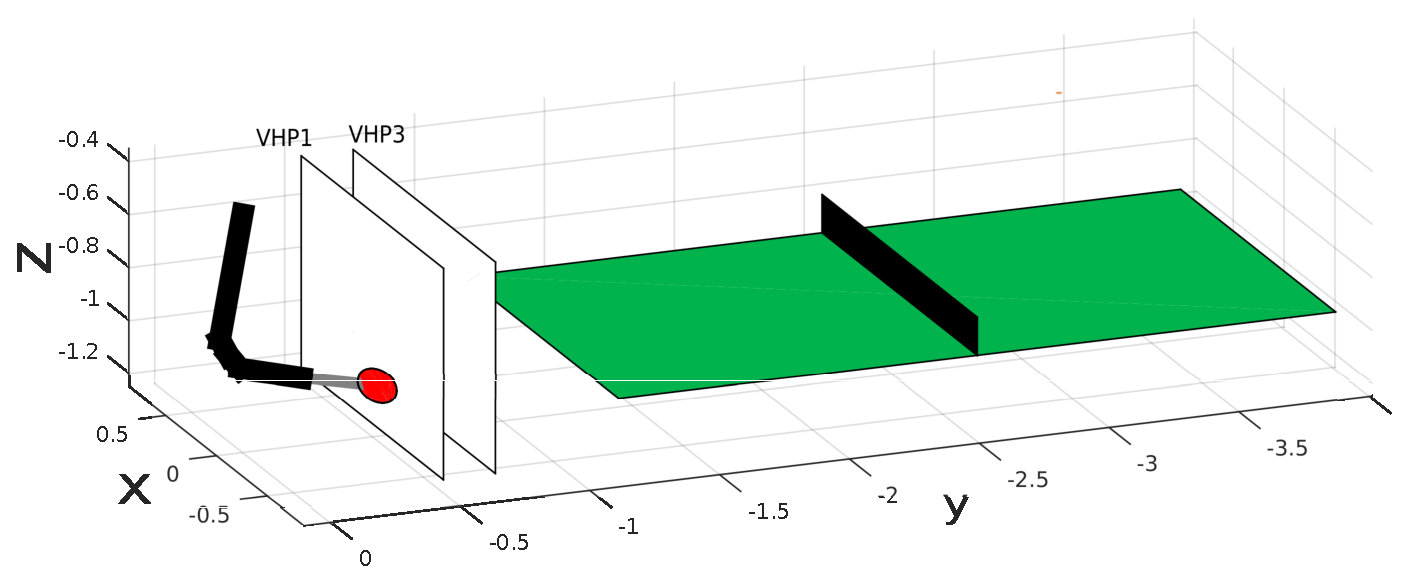
\includegraphics[scale=0.25]{tableTennisVHP.eps}			
\caption{For simulating the performance of the VHP method in a fair way, we average the results over four different VHP locations. The first and third plane locations are shown in the figure. Out of $50$ balls each, the VHP methods with $y = -0.7,-0.6,-0.5,-0.4$ return $31, 37, 28, 29$ balls respectively.}
\label{vhps}
\end{figure}
%
We summarize our evaluations in Table~\ref{tableSimResults}. A total of $200$ balls are launched towards the robot in single-ball solo trials from varying initial positions and velocities. The initial ball mean $\vec{\mu}_{\mathrm{init}}$ is fixed at a sensible value and the covariance is diagonal with a standard deviation of $\sigma_{\mathrm{init}} = 0.1$, i.e. $\ball_{\mathrm{init}} \sim \mathcal{N}(\vec{\mu}_{\mathrm{init}}, \vec{\Sigma}_{\mathrm{init}})$, $\vec{\Sigma}_{\mathrm{init}} = \sigma_{\mathrm{init}}^2 \vec{I}$. Some balls are illegal, for example they might not bounce on the robot's court. Such balls are detected with our ball prediction models and they are not considered for strike generation. They are marked as \emph{Not Valid} in Table~\ref{tableSimResults}. 

Comparing with the VHP method, we see that $\alg$ is able to return more balls to the other side. VHP method suffers from joint limit violations, with $26$ more balls not struck. One of the main reasons for this increase in performance is the fixed location of the VHP. Depending on the incoming ball velocity, a fixed VHP can result in joint limit violations or infeasible solutions. A second reason is the explicit incorporation of joint limits both for the striking trajectory and the return trajectory in our optimization problem. See Figure~\ref{vhps} for an illustration. Out of $50$ balls each, the VHP methods with the planes fixed at $y = -0.7,-0.6,-0.5,-0.4$ locations return $31, 37, 28, 29$ balls respectively. For this particular ball distribution, the plane at $y = -0.7$ seems to be the most robust option.
% talk more on the GP models
% figure needed

% Shall we put a small video for simulations?

\subsection{Robot experiments}

We conduct table tennis experiments in our robotic table tennis setup, see Figure~\ref{robot}. Our custom-made robot is a seven degree of freedom (DoF) Barrett WAM arm that can easily reach $10g$ m/$\textrm{s}^2$ accelerations. It is torque-controlled and cable-driven. A standard size racket ($8$ cm radius) is attached to the end-effector. Our vision system tracks the balls at a rate of $60$ Hz and consists of four cameras on the corners on the ceiling. Each camera provides raw ball data which is first fused together and then filtered with an Extended Kalman Filter (EKF). The table and the tennis balls are standard sized, the balls have a radius of $2$ cm, the table geometry is roughly $276 \times 152 \times 76$ cm.

In our experiments we use a ball-launcher (see Figure~\ref{robot}) to throw balls to the right hand side of the robot. The ball comes with a high variance, especially the velocities are quite unpredictable even without oscillation. The robot is at a distance of roughly $115$ cm. The robots initial posture with a comfortable forehand is chosen after a little experimentation to simplify the trajectory generation task. Other specifications are the same as in our simulation environment. The video shows the feasibility of our approach in practice.

% vision system operates in a semi-structured and human-inhabited environment
% Finite State Automaton: four stages: awaiting stage, preparation, hitting and finishing stage